% --------------------------------------------------------------
%                           Set Up
% --------------------------------------------------------------
 
\documentclass[12pt]{article}
 
\usepackage[margin=1in]{geometry} 
\usepackage{amsmath,amsthm,amssymb}
\usepackage{listings}
\usepackage{xcolor}
\usepackage{graphicx}
\usepackage{subcaption}
\usepackage{listings}
\usepackage{xcolor}
\usepackage{comment}
\usepackage{hepnames}
\usepackage{longtable}
 
\definecolor{codegreen}{rgb}{0,0.6,0}
\definecolor{codegray}{rgb}{0.5,0.5,0.5}
\definecolor{codepurple}{rgb}{0.58,0,0.82}
\definecolor{backcolour}{rgb}{0.95,0.95,0.92}
 
\lstdefinestyle{mystyle}{
    backgroundcolor=\color{backcolour},   
    commentstyle=\color{codegreen},
    keywordstyle=\color{magenta},
    numberstyle=\tiny\color{codegray},
    stringstyle=\color{codepurple},
    basicstyle=\ttfamily\footnotesize,
    breakatwhitespace=false,         
    breaklines=true,                 
    captionpos=b,                    
    keepspaces=true,                 
    numbers=left,                    
    numbersep=5pt,                  
    showspaces=false,                
    showstringspaces=false,
    showtabs=false,                  
    tabsize=2
}
 
\lstset{style=mystyle}
 
\definecolor{codegreen}{rgb}{0,0.6,0}
\definecolor{codegray}{rgb}{0.5,0.5,0.5}
\definecolor{codepurple}{rgb}{0.58,0,0.82}
\definecolor{backcolour}{rgb}{0.95,0.95,0.92}
\definecolor{deepblue}{rgb}{0,0,0.5}
\definecolor{deepred}{rgb}{0.6,0,0}
\definecolor{deepgreen}{rgb}{0,0.5,0}
 
\lstdefinestyle{mystyle}{
    backgroundcolor=\color{backcolour},   
    commentstyle=\color{codegreen},
    keywordstyle=\color{deepred},
    numberstyle=\tiny\color{codegray},
    stringstyle=\color{deepblue},
    basicstyle=\ttfamily\footnotesize,
    breakatwhitespace=false,         
    breaklines=true,                 
    captionpos=b,                    
    keepspaces=true,                 
    numbers=left,                    
    numbersep=5pt,                  
    showspaces=false,                
    showstringspaces=false,
    showtabs=false,                  
    tabsize=2
}
 
\lstset{style=mystyle}
 
\newcommand{\N}{\mathbb{N}}
\newcommand{\Z}{\mathbb{Z}}
 
\newenvironment{theorem}[2][Theorem]{\begin{trivlist}
\item[\hskip \labelsep {\bfseries #1}\hskip \labelsep {\bfseries #2.}]}{\end{trivlist}}
\newenvironment{lemma}[2][Lemma]{\begin{trivlist}
\item[\hskip \labelsep {\bfseries #1}\hskip \labelsep {\bfseries #2.}]}{\end{trivlist}}
\newenvironment{exercise}[2][Exercise]{\begin{trivlist}
\item[\hskip \labelsep {\bfseries #1}\hskip \labelsep {\bfseries #2.}]}{\end{trivlist}}
\newenvironment{problem}[2][Problem]{\begin{trivlist}
\item[\hskip \labelsep {\bfseries #1}\hskip \labelsep {\bfseries #2.}]}{\end{trivlist}}
\newenvironment{question}[2][Question]{\begin{trivlist}
\item[\hskip \labelsep {\bfseries #1}\hskip \labelsep {\bfseries #2.}]}{\end{trivlist}}
\newenvironment{corollary}[2][Corollary]{\begin{trivlist}
\item[\hskip \labelsep {\bfseries #1}\hskip \labelsep {\bfseries #2.}]}{\end{trivlist}}

\newenvironment{solution}{\begin{proof}[Solution]}{\end{proof}}

\setlength\parindent{0pt}
 
\begin{document}
 
% -------------------------------------------------------------- 
%                         Start here
% --------------------------------------------------------------
 
\title{Homework }
\author{Timothy Holmes\\ %replace with your name
PHY 442 Computational Physics}

\maketitle

\section*{Problem 1}

Given the integral,

$$
\int_{0}^{1} \frac{4}{1 + x^2} dx \\
$$

is pretty easy to solve for analytically. Evaluating this integral gives the results

$$
\Big[4 * tan^{-1}(x) \Big]_{0}^{1} = \pi \approx 3.1416. \\
$$

The Monte Carlo method is great for integrals that can not be solved analytically. It is a numerical technique that allows us to get a good enough approximation for what the value of the integral should be, for most cases. Therefore, for our purposes, knowing the actually analytical value of an integral is a good way to check how well our numerical method answer has produced. When testing our program, we should expect a value that is close to $\pi$. If we're far off, that can tell us one of two things. There is a problem in our program or that there is a numerical error. The first step in tackling this problem is to run the randomly generated points from $n = 100$ and varying this number up until $n = 10,000$. The following cases were produced from the monte\_carlo\_average program that can be found in the appendix.\\


\begin{center}
n = 100, regions = 3 \\
Total area: 3.130081 \\
Total error: 0.020132 \\
\end{center}

\begin{center}
n = 1000, regions = 3 \\
Total area: 3.144927 \\
Total error: 0.006049 \\
\end{center}

\begin{center}
n = 3000, regions = 3 \\
Total area: 3.145303 \\
Total error: 0.003571 \\
\end{center}

\begin{center}
n = 6000, regions = 3 \\
Total area: 3.144341 \\
Total error: 0.002525 \\
\end{center}

\begin{center}
n = 10000, regions = 3 \\
Total area: 3.142754 \\
Total error: 0.001952 \\
\end{center}

The most significant change in values occur between the $n = 100$ and $n = 1000$ case. The error changes on one order of magnitude, which should be noted as significant. However, the remaining results are not as interesting. It should be noted that as n increases are error decreases and our values becomes more accurate. From $n = 1000$ to $n = 10000$ the error is essentially divided by $~2$ each time the values of $n$ is multiplied by $2$. The overall takeaway from this experiment, the more $n$ increases the more we can rely on the accuracy of our answer. Knowing the actual result shows that the answers only gave an accurate answer within 2 decimal places. This can then again be improves by increasing the value of $n$ but this will also result in the run-time becoming extremely long. The following figures show the regions and plot points in which the area was calculated from.

\begin{figure}[htp]
\centering

\begin{subfigure}{0.49\columnwidth}
\centering
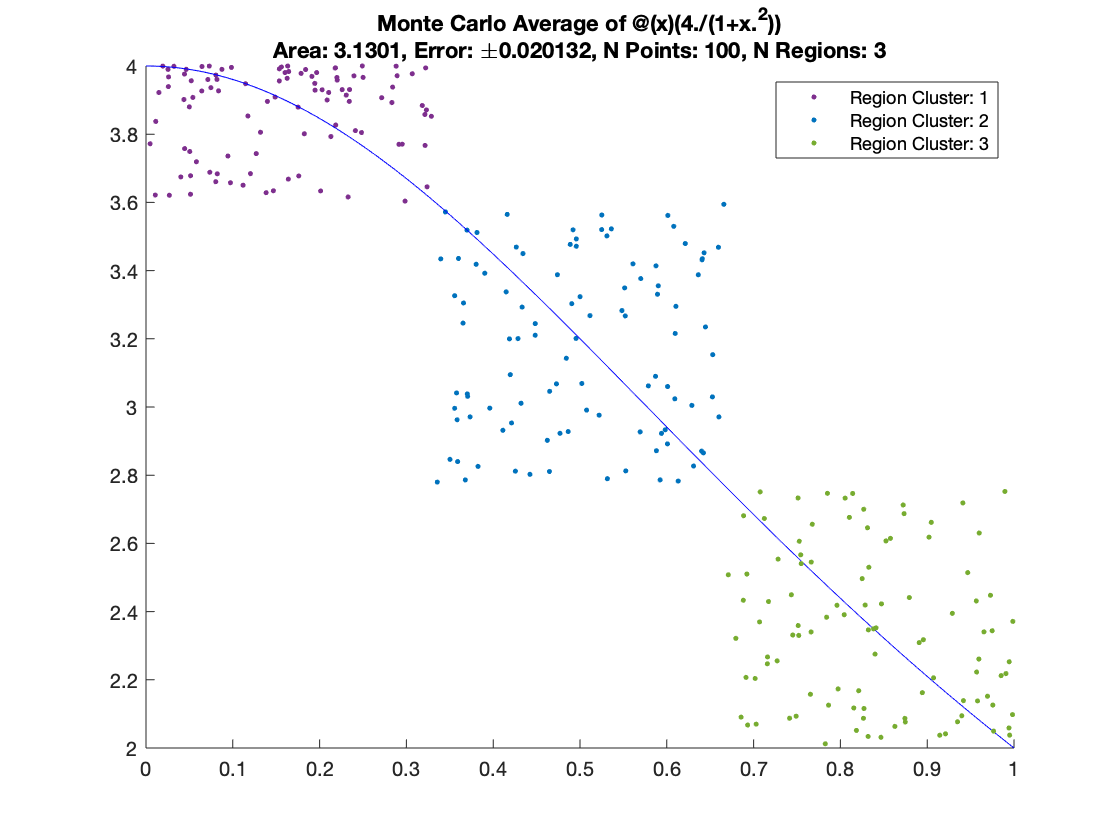
\includegraphics[width=\textwidth]{problem_1_n_100.png}
\caption{}
\label{fig:time1}
\end{subfigure}\hfill
\begin{subfigure}{0.49\columnwidth}
\centering
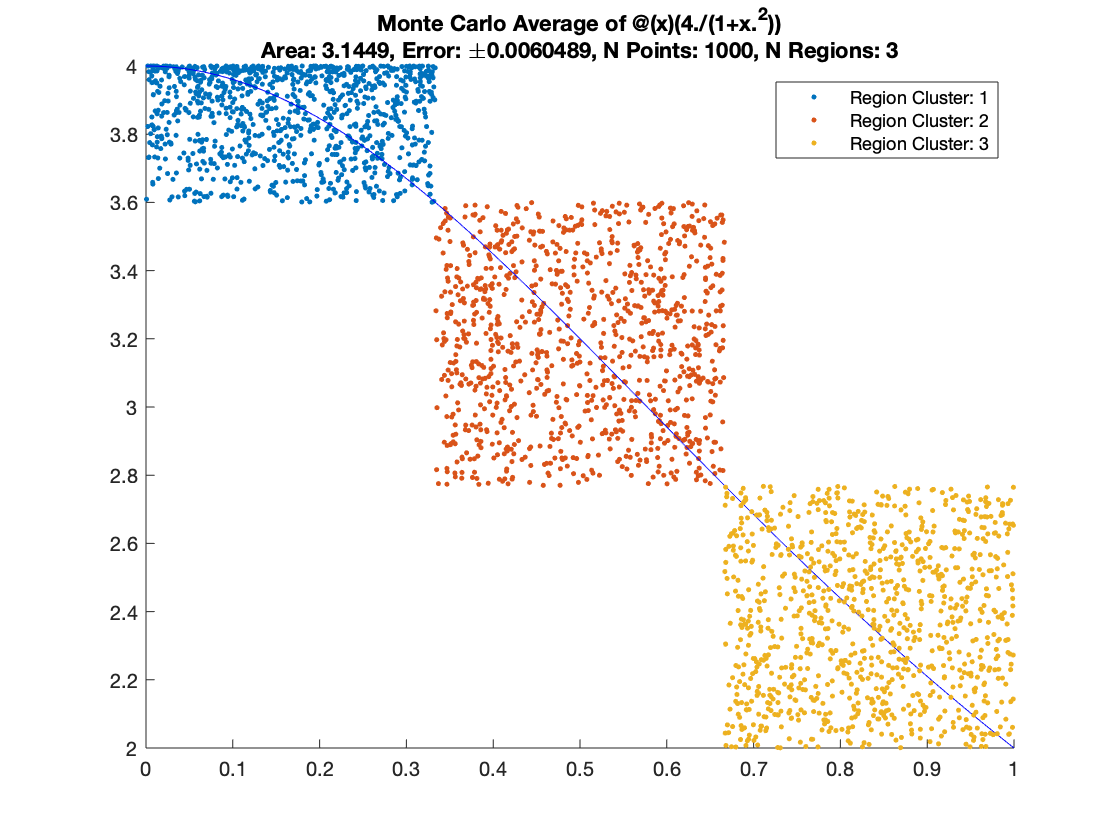
\includegraphics[width=\textwidth]{problem_1_n_1000.png}
\caption{}
\label{fig:time2}
\end{subfigure}

\medskip

\begin{subfigure}{0.49\columnwidth}
\centering
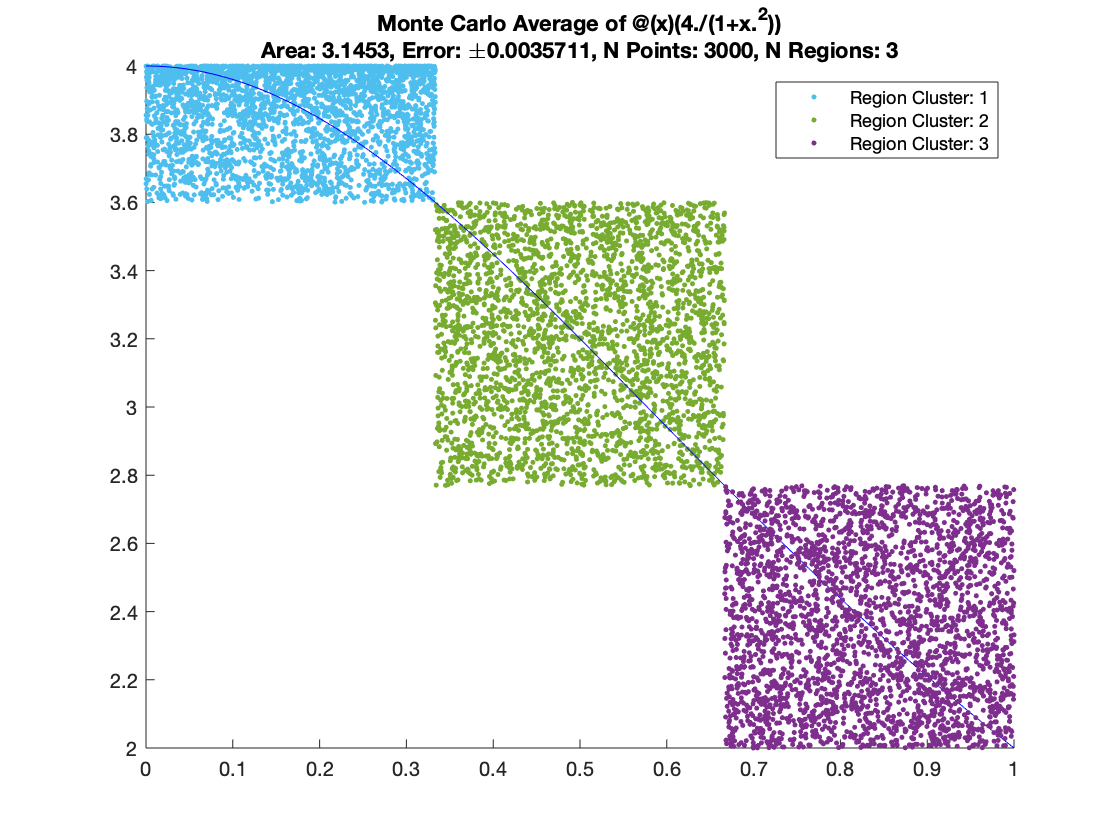
\includegraphics[width=\textwidth]{problem_1_n_3000.png}
\caption{}
\label{fig:time3}
\end{subfigure}\hfill
\begin{subfigure}{0.49\columnwidth}
\centering
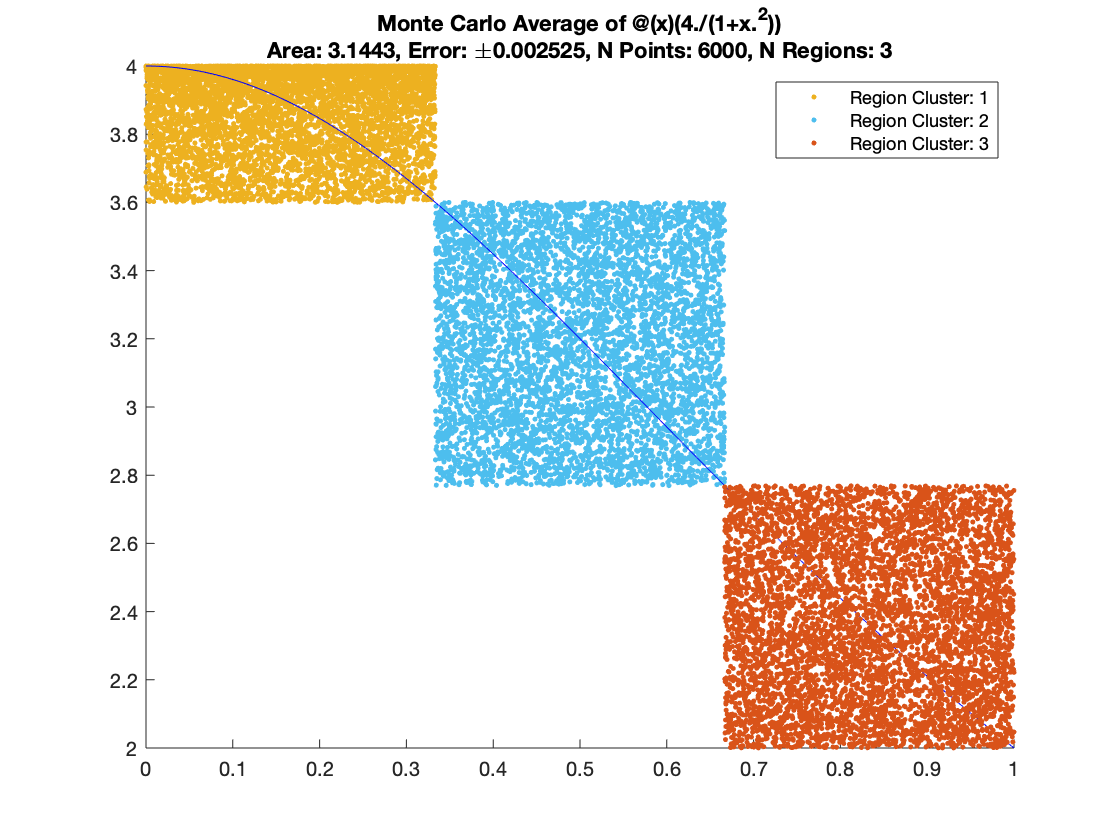
\includegraphics[width=\textwidth]{problem_1_n_6000.png}
\caption{}
\label{fig:time4}
\end{subfigure}

\medskip

\begin{subfigure}{0.49\columnwidth}
\centering
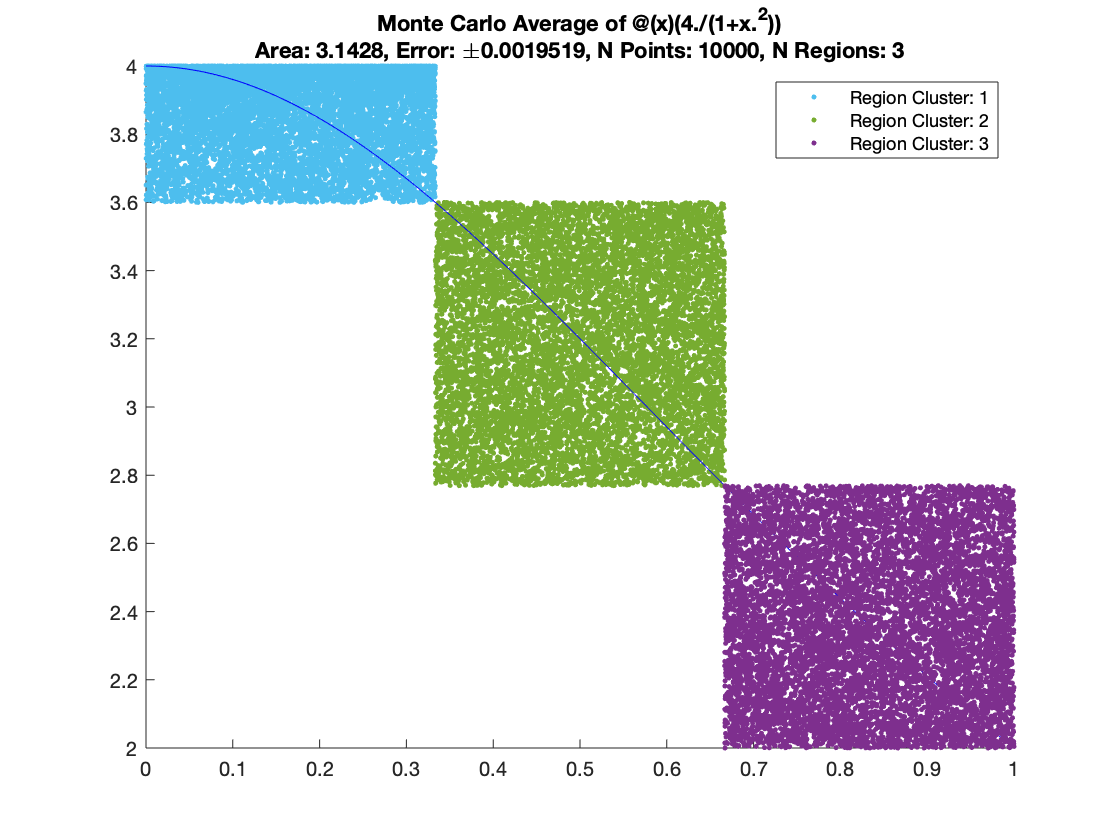
\includegraphics[width=\textwidth]{problem_1_n_10000.png}
\caption{}
\label{fig:time5}
\end{subfigure}

\caption{Various plots from $n = 100$ to $n = 10000$ for 3 regions.}
\label{fig:time}

\end{figure}

\newpage

Now, using the same program but with a different approach yields different answers. Instead of dividing the whole function into regions from $a$ to $b$, this time the Monte Carlo Average will be ran over the whole function. In doing so the program outputs the following

\begin{center}
n = 100, regions = 1 \\
Total area: 3.013535 \\
Total error: 0.065427 \\
\end{center}

\begin{center}
n = 1000, regions = 1 \\
Total area: 3.134747 \\
Total error: 0.020165 \\
\end{center}

\begin{center}
n = 3000, regions = 1 \\
Total area: 3.133269 \\
Total error: 0.011719 \\
\end{center}

\begin{center}
n = 6000, regions = 1 \\
Total area: 3.138856 \\
Total error: 0.008324 \\
\end{center}

\begin{center}
n = 10000, regions = 1 \\
Total area: 3.149766 \\
Total error: 0.006441 \\
\end{center}


There is a lot of information we can extract from this. First, the error values are a lot higher and the total area is much further away from the analytical answer. But this make sense, in the case where $n = 100$ and $region = 1$ the we are limited to just those 100 points. While for the $n = 100$ and $region = 3$ we have in essence 3 different Monte Carlo Area programs running. Where each region has $n = 100$ points. What this really means is that if we divide up the function into 3 regions we really have 300 points. From this we can learn that the number of points can be determined by $total points = n * regions$. Figure 2 below shows the example of the Monte Carlo Average program when there is only one regions.

\begin{figure}[htp]
\centering

\begin{subfigure}{0.49\columnwidth}
\centering
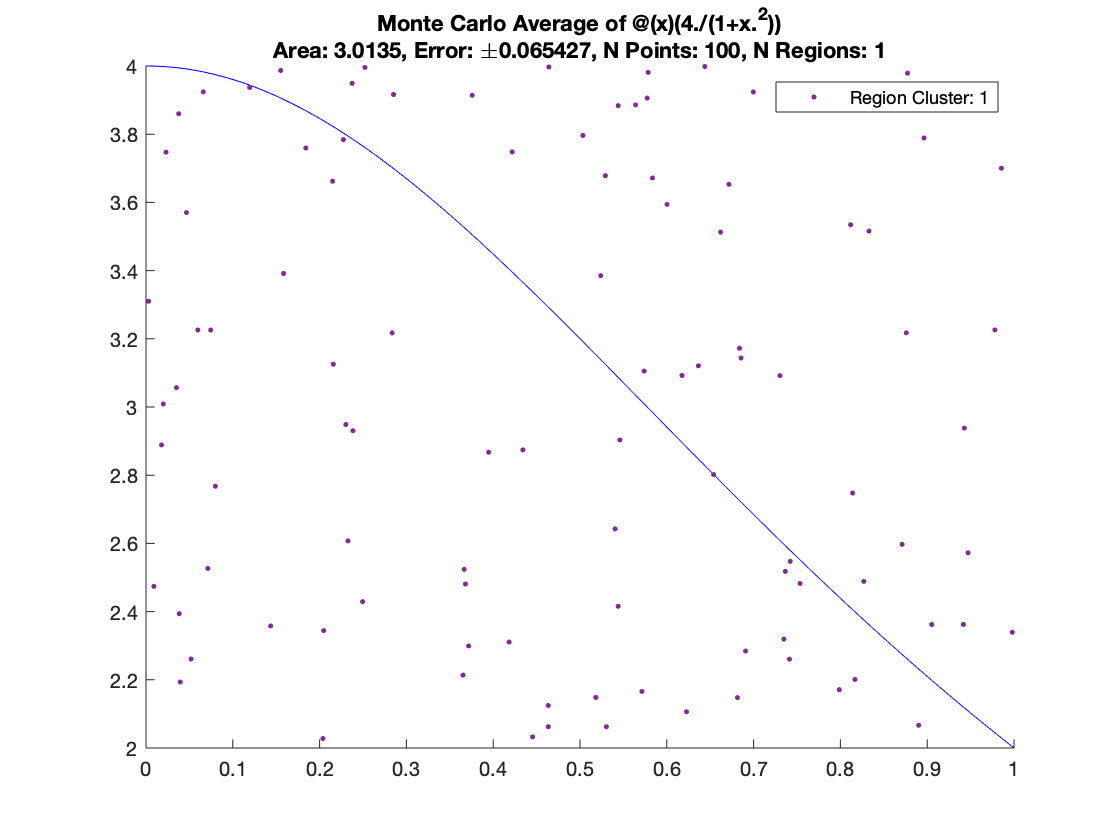
\includegraphics[width=\textwidth]{n_1_region_1.png}
\caption{}
\label{fig:time1}
\end{subfigure}\hfill
\begin{subfigure}{0.49\columnwidth}
\centering
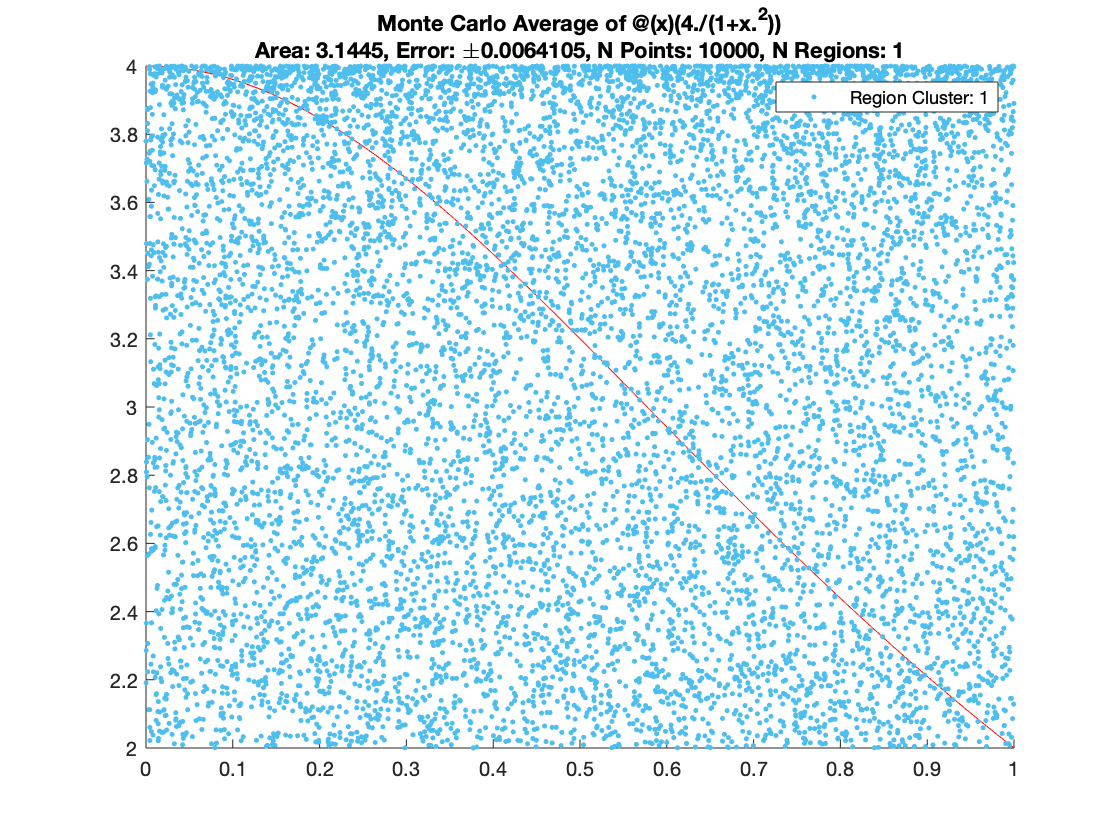
\includegraphics[width=\textwidth]{n_10000_region_1.png}
\caption{}
\label{fig:time2}
\end{subfigure}

\caption{Figure 2 (a) show the program plot when $n = 100$ and there is only one region. Figure 2 (b) show the programs plot when $n = 10000$ and there is only one region selected.}
\label{fig:time}

\end{figure}

\newpage

Finally, there is one more thing we can test with this program. To test the true affect of changing the regions, we will keep the value of points plotted at $n = 5000$ and vary the value of regions from 1 to 4. The program outputs the following

\begin{center}
n = 5000, regions = 1 \\
Total area: 3.149113 \\
Total error: 0.009171 \\
\end{center}

\begin{center}
n = 5000, regions = 2 \\ 
Total area: 3.141429 \\
Total error: 0.004236 \\
\end{center}

\begin{center}
n = 5000, regions = 3 \\
Total area: 3.142770 \\
Total error: 0.002760 \\
\end{center}

\begin{center}
n = 5000, regions = 4 \\
Total area: 3.142844 \\
Total error: 0.002055 \\
\end{center}

Again we see a vary similar outcome from when we varied $n$ points. This is because as previously said, the more regions we add, the more points we add just in different more localized areas of the function. This in returns increases the accuracy of out answer and lowers our error. We see that with each region we add it cuts our error in half. Until a certain point where adding more points simply does not do enough to drastically change the total area. We can think of the Monte Carlo method as a lot of things we interact with in life. The more data and information we have on a system, the better we will understand what is happening and we will get better results. With the same thought process, the more points we plot the closer our estimated area will get to the actual analytical value. The final figure, Figure 3, show how the function looks are the region changes. We see that the density of the plot increases.

\newpage

\begin{figure}[htp]
\centering

\begin{subfigure}{0.49\columnwidth}
\centering
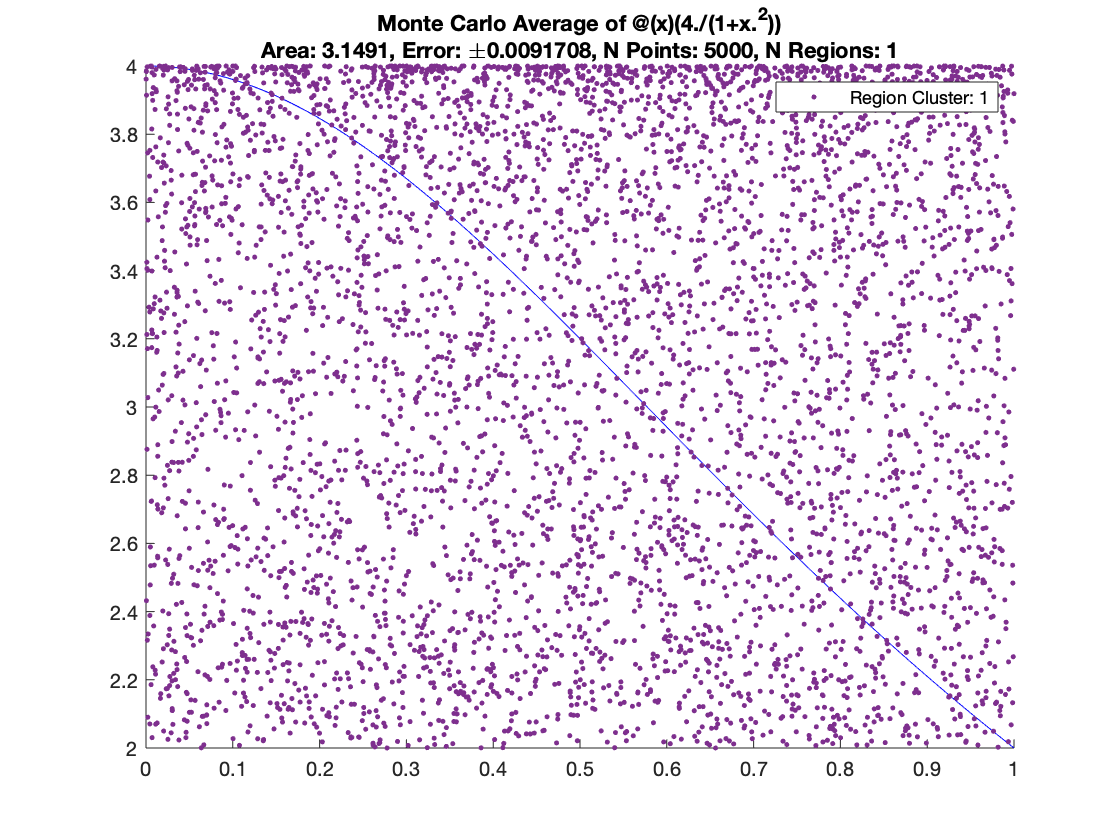
\includegraphics[width=\textwidth]{problem_1_n_5000_reg_1.png}
\caption{}
\label{fig:time1}
\end{subfigure}\hfill
\begin{subfigure}{0.49\columnwidth}
\centering
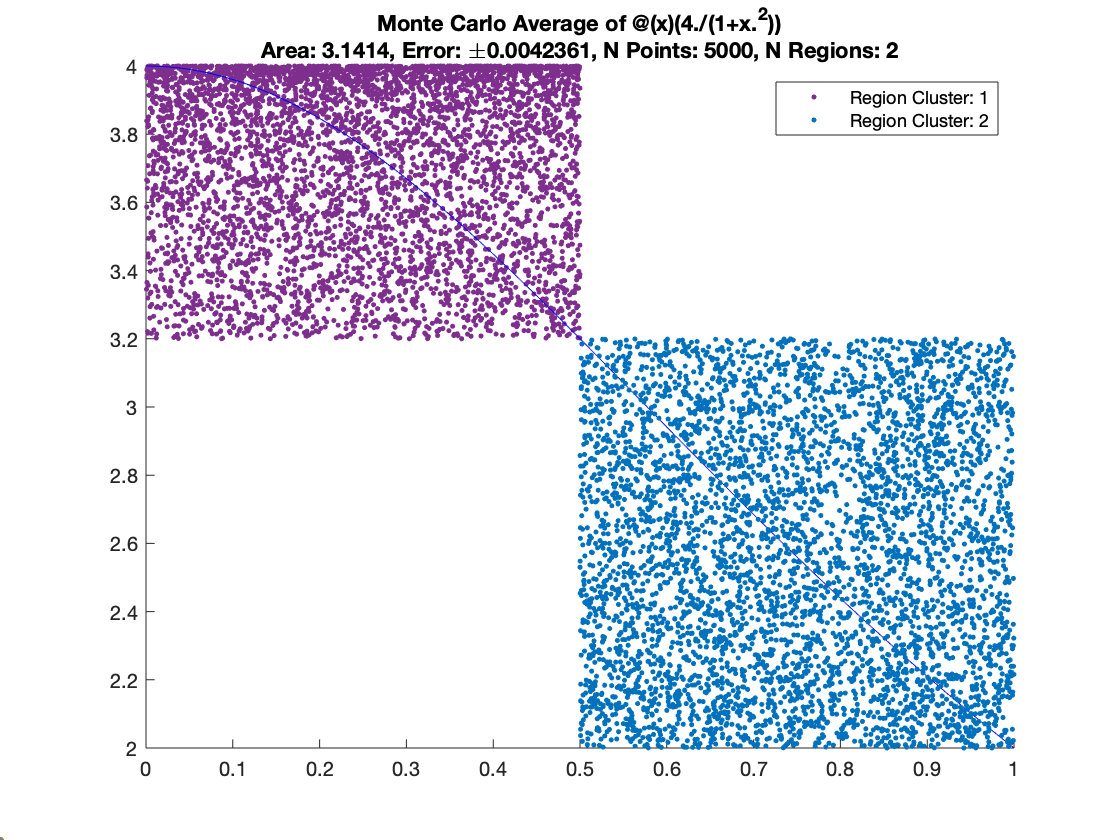
\includegraphics[width=\textwidth]{problem_1_n_5000_reg_2.png}
\caption{}
\label{fig:time2}
\end{subfigure}

\medskip

\begin{subfigure}{0.49\columnwidth}
\centering
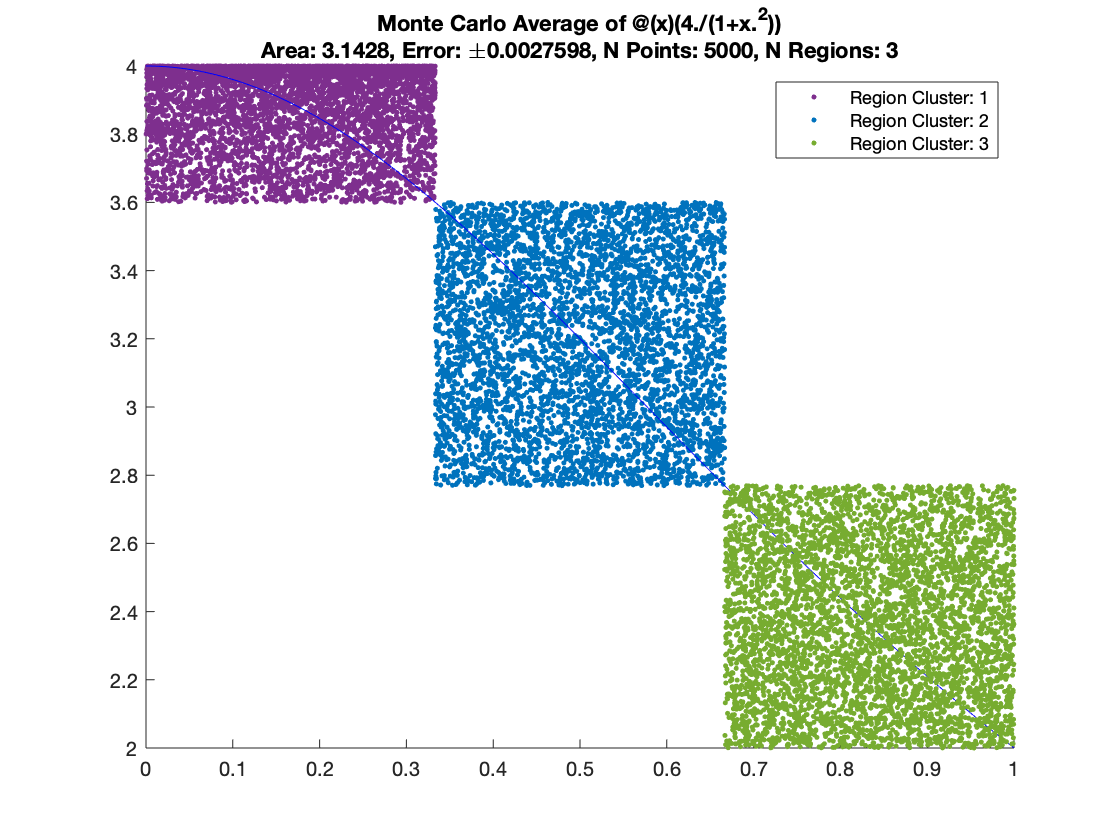
\includegraphics[width=\textwidth]{problem_1_n_5000_reg_3.png}
\caption{}
\label{fig:time3}
\end{subfigure}\hfill
\begin{subfigure}{0.49\columnwidth}
\centering
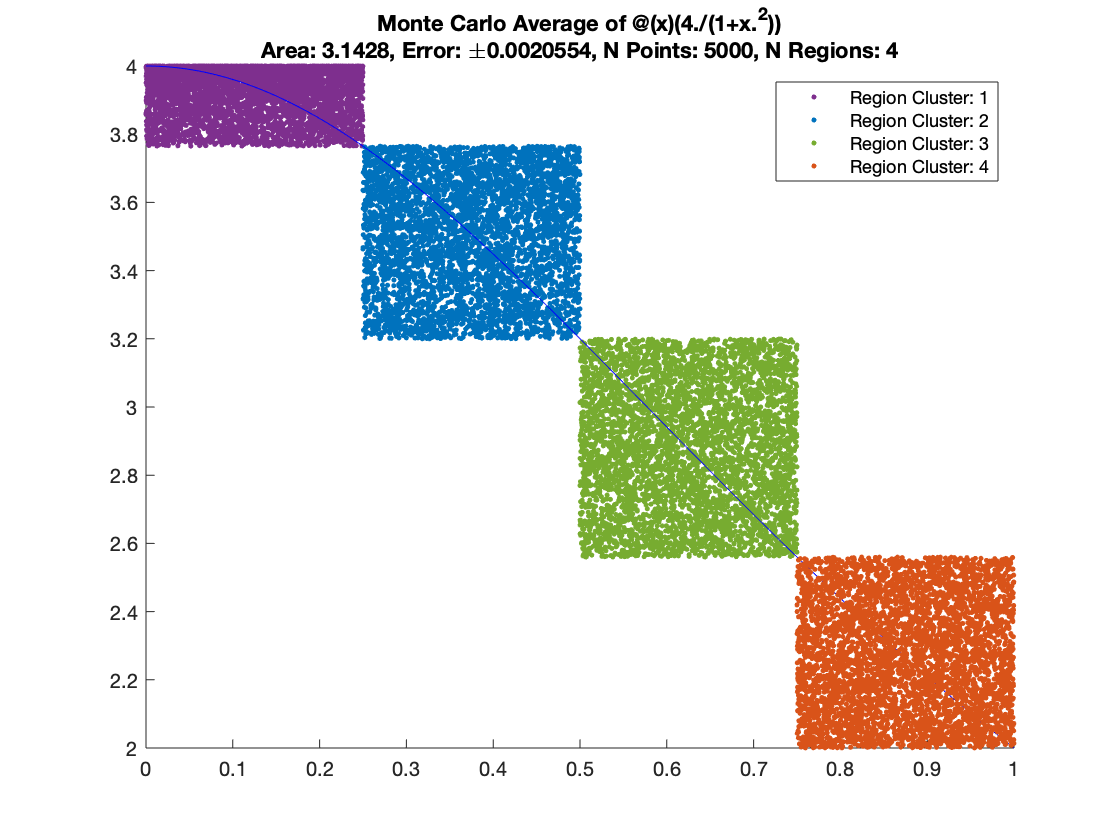
\includegraphics[width=\textwidth]{problem_1_n_5000_reg_4.png}
\caption{}
\label{fig:time4}
\end{subfigure}

\caption{Plots of the Monte Carlo average changing regions from 1 to 4.}
\label{fig:time}

\end{figure}


\newpage

\section*{Problem 2}

The integral is given by

$$
\int_{0}^{1} 4\sqrt{1 - x^{2}} dx
$$

which can be solved analytically by

$$
\Big[2(\sqrt{1 - x^2}x - sin^{-1}(x)  \Big]_{0}^{1} = \pi \approx 3.1416
$$.
 
Using one regions the outputs vary with $n$ points by

\begin{center}
n = 100, regions = 1 \\ 
Total area: 3.098529 \\
Total error: 0.087744 \\
\end{center}

\begin{center}
n = 500, regions = 1 \\
Total area: 3.128460 \\
Total error: 0.041565 \\
\end{center}

\begin{center}
n = 1000, regions = 1 \\
Total area: 3.138487 \\
Total error: 0.028249 \\
\end{center}

Again, we see a similar pattern as we did in problem 1. Each time we double the value of $n$ we half the output of the error. When $n = 100$ none of the decimal points agree. When $n = 500$ and $n = 1000$ only the first decimal place agrees with the analytical value. To have more decimal values agree, the value of $n$ needs to be scaled up, like what was seen in the prior problem.


\section*{Problem 3}

The plots generated were for $N = 100$, $N = 250$, $N =500$. figures are on the next page. As we increase the value of $N$ (Number of collisions) we find that the line of the plot becomes more defined and smooth.

\begin{figure}[htp]
\centering

\begin{subfigure}{0.49\columnwidth}
\centering
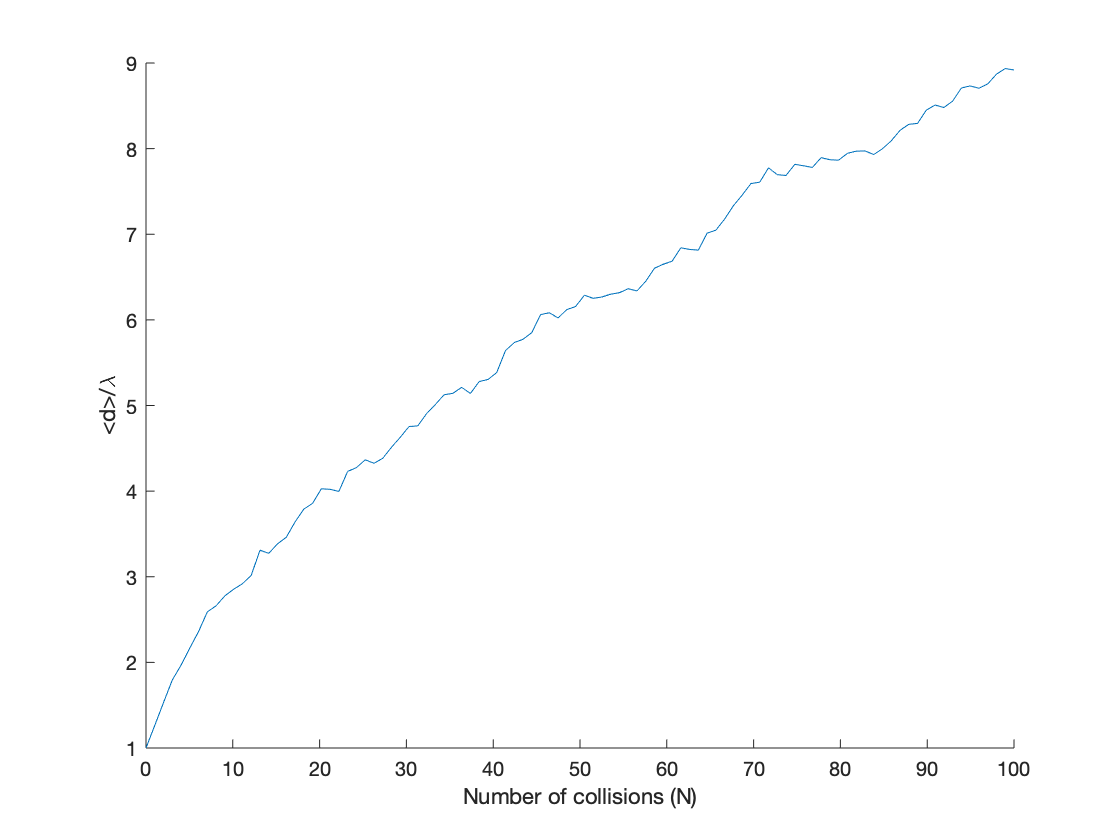
\includegraphics[width=\textwidth]{100.png}
\caption{}
\label{fig:time1}
\end{subfigure}\hfill
\begin{subfigure}{0.49\columnwidth}
\centering
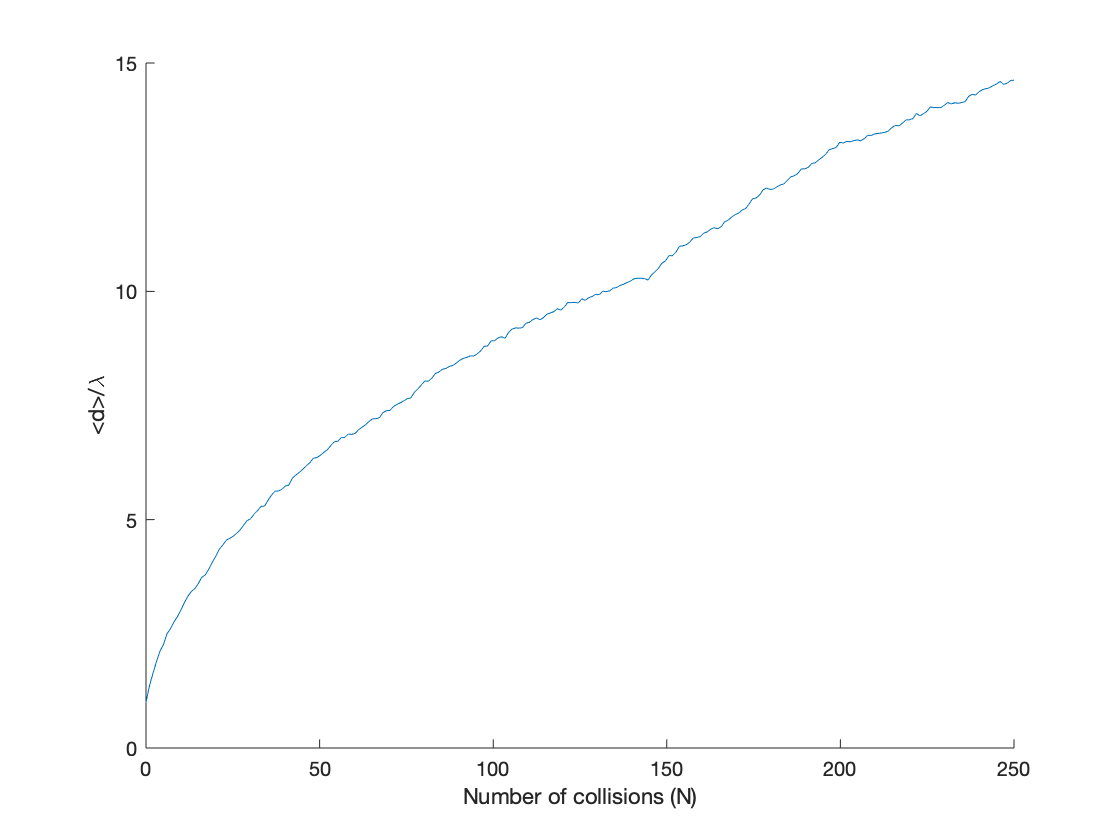
\includegraphics[width=\textwidth]{250.png}
\caption{}
\label{fig:time2}
\end{subfigure}

\medskip

\begin{subfigure}{0.49\columnwidth}
\centering
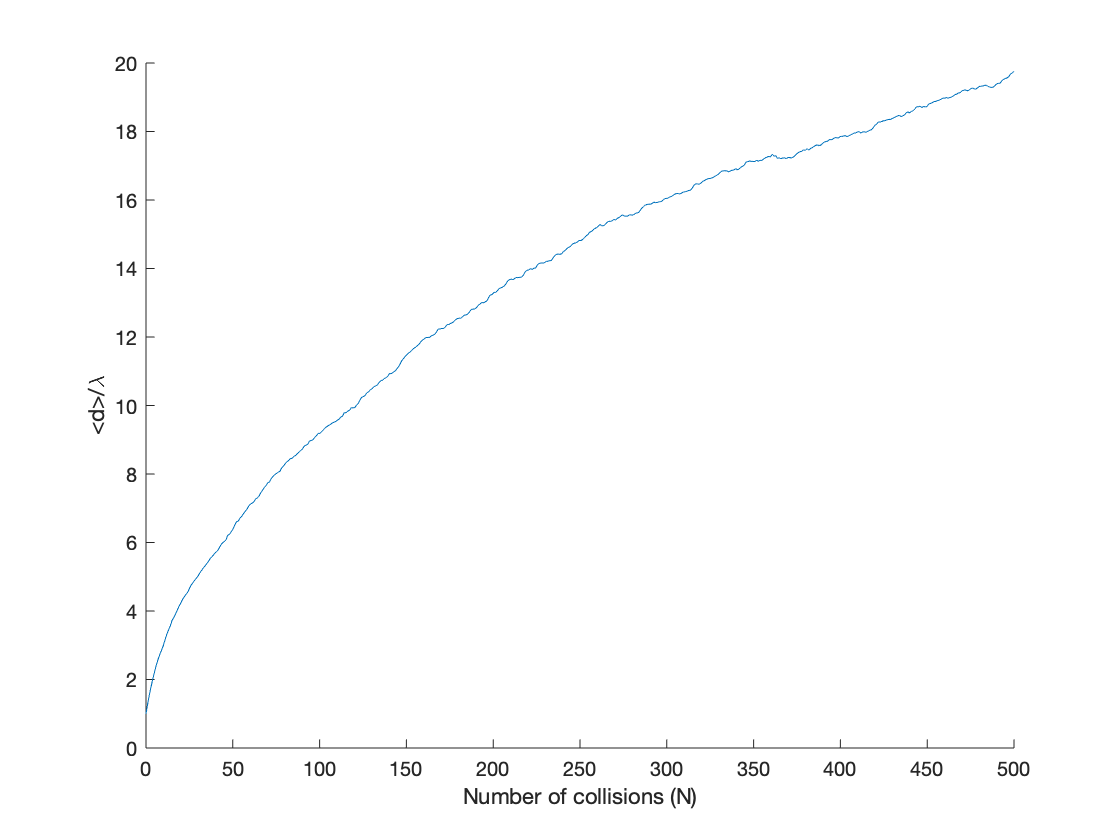
\includegraphics[width=\textwidth]{500.png}
\caption{}
\label{fig:time3}
\end{subfigure}\hfill

\caption{Plots from the Monte Carlo Simulation.}
\label{fig:time}

\end{figure}

\newpage

\section*{Problem 4}

This plot was fitted by a custom program that is shown in the appendix. The following equation was used to fit the graph

\begin{center}
Equation is y = 0.49289*x + -0.0144
\end{center}

where the value of $q = 0.49289$. The graph generated is below. 

\begin{figure}[h!]
    \centering
    {{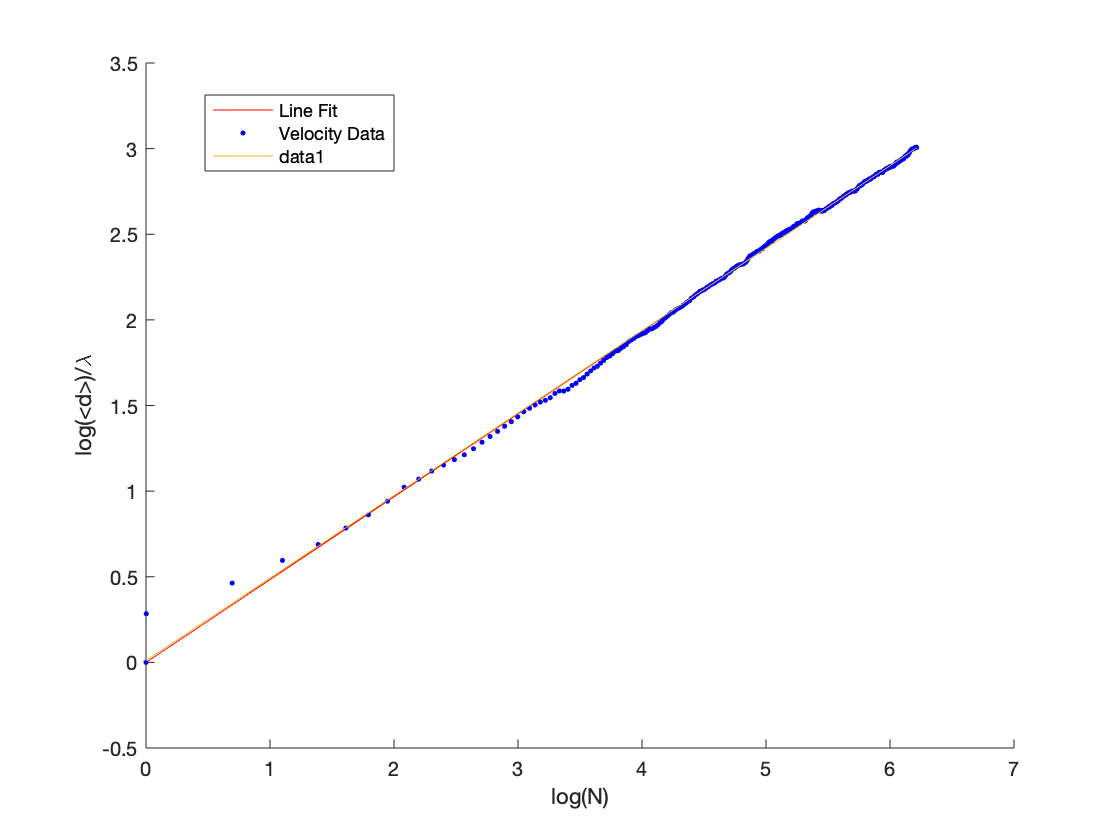
\includegraphics[width=15cm]{log_plot.png}}}%
    \qquad
    \caption{ }%
    \label{fig:example}%
\end{figure}

There are two fitted lines in this plot, one using my program and the other using MATLAB's built in line fit function to confirm accuracy. The value of $q$ does indicate that it is positively correlated. However, this correlation is weak and isn't very likely that it plays a role in the mean free path. 

\section*{Appendix}

\subsection*{Monte Carlo Average}
\begin{lstlisting}[language=Matlab, caption= ]
function monte_carlo_average(g_x, a, b, n_regions, n)
%% Monte Carlo Average
%   - Curve fit
%   
%   Input Arg
%   ---------
%   g_x - function: Default: data
%       Some function
%   a - float: Default: data
%       x_lower_bound
%   b - float: Default: data
%       x_upper_bound
%   n_regions - int: Default: data
%       Number of split regions
%   n - int: 
%       Number of random points
%
%   Optional Input
%   --------------
%   None
%       Runs func that rutens homework 1 Args
%
%   Output Arg
%   ----------
%   p_x - Curve fit plots
%   x   - Original x-axis values
disp('Running')
disp('-------')
if (~exist('g_x', 'var')) && (~exist('a', 'var')) && (~exist('b', 'var')) && (~exist('n_regions', 'var')) && (~exist('n', 'var'))
    [g_x, a, b, n_regions, n] = sample_data(); 
end

region_split = n_regions;
regions = linspace(a, b, (region_split + 1));
m = (length(regions) - 1);

region_length = zeros((length(regions) - 1), 1);
for i = 1:m
    region_length(i) = regions(i + 1) - regions(i);
end

func    = zeros(n, 1);
area    = zeros(m, 1);
func_sq = zeros(n, 1);
error   = zeros(n, 1);
x_line = linspace(a, b, 1000);

fig1 = figure('Visible', 'off');
ax1 = axes('Parent', fig1);
hold(ax1, 'on');
p2 = zeros(m, 1);
legend_info = cell(m, 1);

for i = 1:m
    for j = 1:n
    
    x = regions(i) + (regions(i + 1) - regions(i)) .* rand(j, 1);
    
    func(j) = g_x(x(j));
    func_sq(j) = g_x(x(j))^2;
    
    plot(x(j), func(j))

    end
    
    func_avg = sum(func)/n;
    func_sq_avg = sum(func_sq)/n;
    
    area(i) = func_avg * region_length(i);
  
    error(i) = region_length(i) * sqrt((func_sq_avg - func_avg^2)/n);
    

    plot(ax1, x_line, g_x(x_line), 'r');
    p2(i) = plot(ax1, x, func, '.');
    legend_info{i} = ['Region Cluster: ', num2str(i)]; 
    
end

total_area = sum(area);
fprintf('Total area: %f \n', total_area)

total_error = sum(error);
fprintf('Total error: %f \n', total_error)

%% generate plot
title({['Monte Carlo Average of ', func2str(g_x)]; ['Area: ', num2str(total_area), ', Error: \pm', ...
        num2str(total_error), ', N Points: ', num2str(n), ', N Regions: ', num2str(n_regions)]})
legend(p2(:), legend_info{:})
hold(ax1, 'off');
set(fig1, 'Visible', 'on');
end



function [g_x, a, b, n_regions, n] = sample_data()

% g_x = @(x) (4./(1 + x.^2));
% a = 0; %x_lower_bound
% b = 1;  %x_upper_bound
% n = 10000;
% n_regions = 1;

g_x = @(x) (4 * sqrt(1 - x.^2));
a = 0; %x_lower_bound
b = 1;  %x_upper_bound
n = 1000;
n_regions = 1;

end
\end{lstlisting}

\subsection*{Monte Carlo Simulation}
\begin{lstlisting}[language=Matlab, caption= ]
function monte_carlo_simulation(particles, num_colisions)
%% Cubic Spline
%   - Curve fit
%   
%   Input Arg
%   ---------
%   g_x - funum_colisionstion: Default: data
%       Some funum_colisionstion
%   a - float: Default: data
%       x_lower_bound
%   b - float: Default: data
%       x_upper_bound
%   c - float: Default: data
%       y_lower_bound
%   d - float: Default: data
%       y_upper_bound
%   n - int: 
%       Number of random points
%
%   Optional Input
%   --------------
%   None
%       Runs funum_colisions that rutens homework 1 Args
%
%   Output Arg
%   ----------
%   p_x - Curve fit plots
%   x   - Original x-axis values
disp('Running')
disp('-------')
if (~exist('N', 'var')) && (~exist('p', 'var')) 
    [particles, num_colisions] = sample_data(); 
end

count = 0;
r = 1;
lambda = 1;
dis = zeros(particles, num_colisions);
for i = 1:particles
    x1 = 5;
    y1 = 5;
    z1 = 5;
    count = count + 1;
    for j = 1:num_colisions
  
        theta = acos(-1 + 2*rand);
        %q = cos(theta);
        phi = 2 * pi * rand;
        [x, y, z] = sph2cart(theta, phi, r);
        x1 = x + x1;
        y1 = y + y1;
        z1 = z + z1;
        dis(i, j) = sqrt((x1 - 5)^2 + (y1 - 5)^2 + (z1 - 5)^2);
        if count == num_colisions
            %scatter3(x1, y1, z1, 'MarkerFaceColor', 'k')
            %hold on
        end
    end
end

%% Set equations for figure 1
N = linspace(0, num_colisions, length(dis));
N_q_approx = mean(dis)/lambda;
%dis_approx = N.^q;

%% Plot figure 1
hold on
figure(1)
plot(N, N_q_approx)
xlabel('Number of collisions (N)')
ylabel('<d>/\lambda')

%% Set equations for figure 1
q_ln_N_approx = log(mean(dis)/lambda);
ln_N = log(N);
ln_N(1) = 0;

%% Plot figure 2
hold on
figure(2)
least_square_line_fit(ln_N, q_ln_N_approx, 0, 1)

c = polyfit(ln_N, q_ln_N_approx, 1);
disp(['Equation is y = ' num2str(c(1)) '*x + ' num2str(c(2))])
yfit = c(1) * ln_N + c(2);
plot(ln_N, yfit)
xlabel('log(N)')
ylabel('log(<d>)/\lambda')


end


function [particles, num_colisions] = sample_data()

particles =  500;
num_colisions = 500;

end
\end{lstlisting}

\subsection*{line Fit}
\begin{lstlisting}[language=Matlab, caption= ]
function least_square_line_fit(x, y, sigma_bool, sigma_values)

disp('Running')
disp('-------')
if (~exist('x', 'var')) && (~exist('y', 'var'))
    [x, y, sigma_bool, sigma_values] = homework_2_values(); 
end


if sigma_bool == 1
    fit_type = 'sigma';
    sigma = 0;
    
elseif sigma_bool == 0
    fit_type = 'no_sigma';
    sigma = sigma_values;

else
    warning('Unexpected sigma_values type. Input must be a boolean value.')
end


switch fit_type
    case 'sigma'
        
        s    = sum(1/sigma^2);
        s_x  = sum(x/sigma^2);
        s_y  = sum(y/sigma^2);
        s_xx = sum(x^2/sigma^2);
        s_xy = sum((x * y)/sigma^2);
        
        delta = ((s * s_xx) - (s_x)^2);
        a_1 = ((s_xx * s_y) - (s_x * s_xy))/delta;
        a_2 = ((s * s_xy) - (s_x * s_y))/delta;
        
        a_1_variance = s_xx/delta;
        a_2_variance = s/delta;
        
        fprintf('Error in a_1: %f \n', a_1_variance)
        fprintf('Error in a_2: %f \n', a_2_variance)
        
        
    case 'no_sigma'
        
        n    = length(x);
        s    = sum(1/sigma^2);
        s_x  = sum(x/sigma^2);
        s_y  = sum(y/sigma^2);
        s_xx = sum(x.^2/sigma^2);
        s_xy = sum((x .* y)/sigma^2);
        
        delta = ((s * s_xx) - (s_x)^2);
        a_1   = ((s_xx * s_y) - (s_x * s_xy))/delta;
        a_2   = ((s * s_xy) - (s_x * s_y))/delta;
        
        chi = sum(((y - a_1 - (a_2 * x))/sigma).^2);
        
        a_1_variance = s_xx/delta;
        a_2_variance = s/delta;
        
        a_1_error = a_1_variance * (chi^2/(n - 2)^(1/2));
        a_2_error = a_2_variance * (chi^2/(n - 2)^(1/2));
        
        fprintf('Error in a_1: %f \n', a_1_error)
        fprintf('Error in a_2: %f \n', a_2_error)
        
        
    otherwise
        warning('Unexpected fit type. No fit created.')
        
end

plot_fit(x, y, a_1, a_2)

disp('Done.')

end


function plot_fit(x, y, a_1, a_2)
y_fit = a_2 * x + a_1; 
%f_v = a_1 * y + a_2 * y.^2
disp(['Equation is y = ' num2str(a_2) '*x + ' num2str(a_1)])
hold on
plot(x, y_fit, 'r-')
plot(x, y, 'b.')
legend('Line Fit', 'Velocity Data')

end
\end{lstlisting}

% --------------------------------------------------------------
%                           End Document.
% --------------------------------------------------------------
 
\end{document}

